% Options for packages loaded elsewhere
% Options for packages loaded elsewhere
\PassOptionsToPackage{unicode}{hyperref}
\PassOptionsToPackage{hyphens}{url}
\PassOptionsToPackage{dvipsnames,svgnames,x11names}{xcolor}
%
\documentclass[
  twoside,
  symmetric]{tufte-book}
\usepackage{xcolor}
\usepackage{amsmath,amssymb}
\setcounter{secnumdepth}{-\maxdimen} % remove section numbering
\usepackage{iftex}
\ifPDFTeX
  \usepackage[T1]{fontenc}
  \usepackage[utf8]{inputenc}
  \usepackage{textcomp} % provide euro and other symbols
\else % if luatex or xetex
  \usepackage{unicode-math} % this also loads fontspec
  \defaultfontfeatures{Scale=MatchLowercase}
  \defaultfontfeatures[\rmfamily]{Ligatures=TeX,Scale=1}
\fi
\usepackage{lmodern}
\ifPDFTeX\else
  % xetex/luatex font selection
\fi
% Use upquote if available, for straight quotes in verbatim environments
\IfFileExists{upquote.sty}{\usepackage{upquote}}{}
\IfFileExists{microtype.sty}{% use microtype if available
  \usepackage[]{microtype}
  \UseMicrotypeSet[protrusion]{basicmath} % disable protrusion for tt fonts
}{}
\makeatletter
\@ifundefined{KOMAClassName}{% if non-KOMA class
  \IfFileExists{parskip.sty}{%
    \usepackage{parskip}
  }{% else
    \setlength{\parindent}{0pt}
    \setlength{\parskip}{6pt plus 2pt minus 1pt}}
}{% if KOMA class
  \KOMAoptions{parskip=half}}
\makeatother
% Make \paragraph and \subparagraph free-standing
\makeatletter
\ifx\paragraph\undefined\else
  \let\oldparagraph\paragraph
  \renewcommand{\paragraph}{
    \@ifstar
      \xxxParagraphStar
      \xxxParagraphNoStar
  }
  \newcommand{\xxxParagraphStar}[1]{\oldparagraph*{#1}\mbox{}}
  \newcommand{\xxxParagraphNoStar}[1]{\oldparagraph{#1}\mbox{}}
\fi
\ifx\subparagraph\undefined\else
  \let\oldsubparagraph\subparagraph
  \renewcommand{\subparagraph}{
    \@ifstar
      \xxxSubParagraphStar
      \xxxSubParagraphNoStar
  }
  \newcommand{\xxxSubParagraphStar}[1]{\oldsubparagraph*{#1}\mbox{}}
  \newcommand{\xxxSubParagraphNoStar}[1]{\oldsubparagraph{#1}\mbox{}}
\fi
\makeatother


\usepackage{longtable,booktabs,array}
\usepackage{calc} % for calculating minipage widths
% Correct order of tables after \paragraph or \subparagraph
\usepackage{etoolbox}
\makeatletter
\patchcmd\longtable{\par}{\if@noskipsec\mbox{}\fi\par}{}{}
\makeatother
% Allow footnotes in longtable head/foot
\IfFileExists{footnotehyper.sty}{\usepackage{footnotehyper}}{\usepackage{footnote}}
\makesavenoteenv{longtable}
\usepackage{graphicx}
\makeatletter
\newsavebox\pandoc@box
\newcommand*\pandocbounded[1]{% scales image to fit in text height/width
  \sbox\pandoc@box{#1}%
  \Gscale@div\@tempa{\textheight}{\dimexpr\ht\pandoc@box+\dp\pandoc@box\relax}%
  \Gscale@div\@tempb{\linewidth}{\wd\pandoc@box}%
  \ifdim\@tempb\p@<\@tempa\p@\let\@tempa\@tempb\fi% select the smaller of both
  \ifdim\@tempa\p@<\p@\scalebox{\@tempa}{\usebox\pandoc@box}%
  \else\usebox{\pandoc@box}%
  \fi%
}
% Set default figure placement to htbp
\def\fps@figure{htbp}
\makeatother


% definitions for citeproc citations
\NewDocumentCommand\citeproctext{}{}
\NewDocumentCommand\citeproc{mm}{%
  \begingroup\def\citeproctext{#2}\cite{#1}\endgroup}
\makeatletter
 % allow citations to break across lines
 \let\@cite@ofmt\@firstofone
 % avoid brackets around text for \cite:
 \def\@biblabel#1{}
 \def\@cite#1#2{{#1\if@tempswa , #2\fi}}
\makeatother
\newlength{\cslhangindent}
\setlength{\cslhangindent}{1.5em}
\newlength{\csllabelwidth}
\setlength{\csllabelwidth}{3em}
\newenvironment{CSLReferences}[2] % #1 hanging-indent, #2 entry-spacing
 {\begin{list}{}{%
  \setlength{\itemindent}{0pt}
  \setlength{\leftmargin}{0pt}
  \setlength{\parsep}{0pt}
  % turn on hanging indent if param 1 is 1
  \ifodd #1
   \setlength{\leftmargin}{\cslhangindent}
   \setlength{\itemindent}{-1\cslhangindent}
  \fi
  % set entry spacing
  \setlength{\itemsep}{#2\baselineskip}}}
 {\end{list}}
\usepackage{calc}
\newcommand{\CSLBlock}[1]{\hfill\break\parbox[t]{\linewidth}{\strut\ignorespaces#1\strut}}
\newcommand{\CSLLeftMargin}[1]{\parbox[t]{\csllabelwidth}{\strut#1\strut}}
\newcommand{\CSLRightInline}[1]{\parbox[t]{\linewidth - \csllabelwidth}{\strut#1\strut}}
\newcommand{\CSLIndent}[1]{\hspace{\cslhangindent}#1}



\setlength{\emergencystretch}{3em} % prevent overfull lines

\providecommand{\tightlist}{%
  \setlength{\itemsep}{0pt}\setlength{\parskip}{0pt}}



 


\usepackage{lipsum}
\usepackage{booktabs}
\usepackage{graphicx}
\setkeys{Gin}{width=\linewidth,totalheight=\textheight,keepaspectratio}
\graphicspath{{style-guide/graphics/}}
\usepackage{fancyvrb}
\fvset{fontsize=\normalsize}
\newcommand{\hangp}[1]{\makebox[0pt][r]{(}#1\makebox[0pt][l]{)}}
\newcommand{\hangstar}{\makebox[0pt][l]{*}}
\usepackage{xspace}
\newcommand{\vdqi}{\textit{VDQI}\xspace}
\newcommand{\ei}{\textit{EI}\xspace}
\newcommand{\ve}{\textit{VE}\xspace}
\newcommand{\be}{\textit{BE}\xspace}
\newcommand{\VDQI}{\textit{The Visual Display of Quantitative Information}\xspace}
\newcommand{\EI}{\textit{Envisioning Information}\xspace}
\newcommand{\VE}{\textit{Visual Explanations}\xspace}
\newcommand{\BE}{\textit{Beautiful Evidence}\xspace}
\newcommand{\TL}{Tufte-\LaTeX\xspace}
\newcommand{\monthyear}{%
  \ifcase\month\or January\or February\or March\or April\or May\or June\or
  July\or August\or September\or October\or November\or
  December\fi\space\number\year
}
\newcommand{\openepigraph}[2]{%
  \begin{fullwidth}
  \sffamily\large
  \begin{doublespace}
  \noindent\allcaps{#1}\\
  \noindent\allcaps{#2}
  \end{doublespace}
  \end{fullwidth}
}
\newcommand{\blankpage}{\newpage\hbox{}\thispagestyle{empty}\newpage}
\usepackage{units}
\newcommand{\measure}[3]{#1/#2$\times$\unit[#3]{pc}}
\usepackage{makeidx}
\makeindex
\makeatletter
\@ifpackageloaded{caption}{}{\usepackage{caption}}
\AtBeginDocument{%
\ifdefined\contentsname
  \renewcommand*\contentsname{Table of contents}
\else
  \newcommand\contentsname{Table of contents}
\fi
\ifdefined\listfigurename
  \renewcommand*\listfigurename{List of Figures}
\else
  \newcommand\listfigurename{List of Figures}
\fi
\ifdefined\listtablename
  \renewcommand*\listtablename{List of Tables}
\else
  \newcommand\listtablename{List of Tables}
\fi
\ifdefined\figurename
  \renewcommand*\figurename{Figure}
\else
  \newcommand\figurename{Figure}
\fi
\ifdefined\tablename
  \renewcommand*\tablename{Table}
\else
  \newcommand\tablename{Table}
\fi
}
\@ifpackageloaded{float}{}{\usepackage{float}}
\floatstyle{ruled}
\@ifundefined{c@chapter}{\newfloat{codelisting}{h}{lop}}{\newfloat{codelisting}{h}{lop}[chapter]}
\floatname{codelisting}{Listing}
\newcommand*\listoflistings{\listof{codelisting}{List of Listings}}
\makeatother
\makeatletter
\makeatother
\makeatletter
\@ifpackageloaded{caption}{}{\usepackage{caption}}
\@ifpackageloaded{subcaption}{}{\usepackage{subcaption}}
\makeatother
\makeatletter
\@ifpackageloaded{sidenotes}{}{\usepackage{sidenotes}}
\@ifpackageloaded{marginnote}{}{\usepackage{marginnote}}
\makeatother
\usepackage{bookmark}
\IfFileExists{xurl.sty}{\usepackage{xurl}}{} % add URL line breaks if available
\urlstyle{same}
\hypersetup{
  pdftitle={A Tufte-Style Book},
  pdfauthor={The Tufte-LaTeX Developers},
  colorlinks=true,
  linkcolor={blue},
  filecolor={Maroon},
  citecolor={Blue},
  urlcolor={Blue},
  pdfcreator={LaTeX via pandoc}}


\title{A Tufte-Style Book}
\usepackage{etoolbox}
\makeatletter
\providecommand{\subtitle}[1]{% add subtitle to \maketitle
  \apptocmd{\@title}{\par {\large #1 \par}}{}{}
}
\makeatother
\subtitle{Thanks to Edward R. Tufte for his inspiration}
\author{The Tufte-LaTeX Developers}
\date{2025-05-24}
\begin{document}
\frontmatter
\maketitle


\mainmatter
The public is more familiar with bad design than good design. It is, in
effect, conditioned to prefer bad design, because that is what it lives
with. The new becomes threatening, the old reassuring.

-- Paul Rand

A designer knows that he has achieved perfection not when there is
nothing left to add, but when there is nothing left to take away.

-- Antoine de Saint-Exupéry

\ldots the designer of a new system must not only be the implementor and
the first large-scale user; the designer should also write the first
user manual\ldots{} If I had not participated fully in all these
activities, literally hundreds of improvements would never have been
made, because I would never have thought of them or perceived why they
were important.

-- Donald E. Knuth

\chapter*{Introduction}\label{introduction}
\addcontentsline{toc}{chapter}{Introduction}

This sample book discusses the design of Edward Tufte's books(Tufte
2001, 1990, 1997, 2006) and the use of the \texttt{tufte-book} and
\texttt{tufte-handout} document classes.

\chapter{The Design of Tufte's Books}\label{ch:tufte-design}

\footnote{The pages} of a book are usually divided into three major
sections: the front matter (also called preliminary matter or prelim),
the main matter (the core text of the book), and the back matter (or end
matter).

\footnote{The front matter} of a book refers to all of the material that
comes before the main text. The following table shows a list of material
that appears in the front matter of (\textbf{VDQI?}), (\textbf{EI?}),
(\textbf{VE?}), and (\textbf{BE?}) along with its page number. Page
numbers that appear in parentheses refer to folios that do not have a
printed page number (but they are still counted in the page number
sequence).

\begin{longtable}[]{@{}
  >{\raggedright\arraybackslash}p{(\linewidth - 8\tabcolsep) * \real{0.3889}}
  >{\centering\arraybackslash}p{(\linewidth - 8\tabcolsep) * \real{0.1944}}
  >{\centering\arraybackslash}p{(\linewidth - 8\tabcolsep) * \real{0.1389}}
  >{\centering\arraybackslash}p{(\linewidth - 8\tabcolsep) * \real{0.1389}}
  >{\centering\arraybackslash}p{(\linewidth - 8\tabcolsep) * \real{0.1389}}@{}}
\caption{Front matter pages across Tufte's books}\tabularnewline
\toprule\noalign{}
\begin{minipage}[b]{\linewidth}\raggedright
Page content
\end{minipage} & \begin{minipage}[b]{\linewidth}\centering
(\textbf{vdqi?})
\end{minipage} & \begin{minipage}[b]{\linewidth}\centering
(\textbf{ei?})
\end{minipage} & \begin{minipage}[b]{\linewidth}\centering
(\textbf{ve?})
\end{minipage} & \begin{minipage}[b]{\linewidth}\centering
(\textbf{be?})
\end{minipage} \\
\midrule\noalign{}
\endfirsthead
\toprule\noalign{}
\begin{minipage}[b]{\linewidth}\raggedright
Page content
\end{minipage} & \begin{minipage}[b]{\linewidth}\centering
(\textbf{vdqi?})
\end{minipage} & \begin{minipage}[b]{\linewidth}\centering
(\textbf{ei?})
\end{minipage} & \begin{minipage}[b]{\linewidth}\centering
(\textbf{ve?})
\end{minipage} & \begin{minipage}[b]{\linewidth}\centering
(\textbf{be?})
\end{minipage} \\
\midrule\noalign{}
\endhead
\bottomrule\noalign{}
\endlastfoot
Blank half title page & (1) & (1) & (1) & (1) \\
Frontispiece\footnote{The contents of this page vary from book to book.
  In (\textbf{vdqi?}) this page is blank; in (\textbf{ei?}) and
  (\textbf{ve?}) this page holds a frontispiece; and in (\textbf{be?})
  this page contains three epigraphs.} & (2) & (2) & (2) & (2) \\
Full title page & (3) & (3) & (3) & (3) \\
Copyright page & (4) & (4) & (4) & (4) \\
Contents & (5) & (5) & (5) & (5) \\
Dedication & (6) & (7) & (7) & 7 \\
Epigraph & -- & -- & (8) & -- \\
Introduction & (7) & (9) & (9) & 9 \\
\end{longtable}

The design of the front matter in Tufte's books varies slightly from the
traditional design of front matter. First, the pages in front matter are
traditionally numbered with lowercase roman numerals (e.g., i, ii, iii,
iv, \ldots). Second, the front matter page numbering sequence is usually
separate from the main matter page numbering. That is, the page numbers
restart at 1 when the main matter begins. In contrast, Tufte has
enumerated his pages with arabic numerals that share the same page
counting sequence as the main matter.

\section{Typefaces}\label{sec:typefaces1}

Tufte's books primarily use two typefaces: Bembo and Gill Sans. Bembo is
used for the headings and body text, while Gill Sans is used for the
title page and opening epigraphs in (\textbf{BE?}).

Since neither Bembo nor Gill Sans are available in default LaTeX
installations, the Tufte-LaTeX document classes default to using
Palatino and Helvetica, respectively. In addition, the Bera Mono
typeface is used for \texttt{monospaced} type.

The following font sizes are defined by the Tufte-LaTeX classes:

\begin{longtable}[]{@{}lccl@{}}
\caption{LaTeX font sizes as defined by the Tufte-LaTeX document classes
\{\#tbl:font-sizes\}}\tabularnewline
\toprule\noalign{}
LaTeX size & Font size & Leading & Used for \\
\midrule\noalign{}
\endfirsthead
\toprule\noalign{}
LaTeX size & Font size & Leading & Used for \\
\midrule\noalign{}
\endhead
\bottomrule\noalign{}
\endlastfoot
\texttt{\textbackslash{}tiny} & 5 & 6 & sidenote numbers \\
\texttt{\textbackslash{}scriptsize} & 7 & 8 & -- \\
\texttt{\textbackslash{}footnotesize} & 8 & 10 & sidenotes, captions \\
\texttt{\textbackslash{}small} & 9 & 12 & quote, quotation, and verse
environments \\
\texttt{\textbackslash{}normalsize} & 10 & 14 & body text \\
\texttt{\textbackslash{}large} & 11 & 15 & \textbf{B}-heads \\
\texttt{\textbackslash{}Large} & 12 & 16 & \textbf{A}-heads, TOC
entries, author, date \\
\texttt{\textbackslash{}LARGE} & 14 & 18 & handout title \\
\texttt{\textbackslash{}huge} & 20 & 30 & chapter heads \\
\texttt{\textbackslash{}Huge} & 24 & 36 & part titles \\
\end{longtable}

\section{Headings}\label{sec:headings1}

Tufte's books include the following heading levels: parts,
chapters\footnote{Parts and chapters are defined for the
  \texttt{tufte-book} class only.}, sections, subsections, and
paragraphs. Not defined by default are: sub-subsections and
subparagraphs.

\begin{longtable}[]{@{}lll@{}}
\caption{Heading styles used in (\textbf{BE?})
\{\#tbl:heading-styles\}}\tabularnewline
\toprule\noalign{}
Heading & Style & Size \\
\midrule\noalign{}
\endfirsthead
\toprule\noalign{}
Heading & Style & Size \\
\midrule\noalign{}
\endhead
\bottomrule\noalign{}
\endlastfoot
Part & roman & 24/36×40 pc \\
Chapter & italic & 20/30×40 pc \\
Section & italic & 12/16×26 pc \\
Subsection & italic & 11/15×26 pc \\
Paragraph & italic & 10/14 \\
\end{longtable}

\subsection*{Paragraph}\label{paragraph}
\addcontentsline{toc}{subsection}{Paragraph}

Paragraph headings (as shown here) are introduced by italicized text and
separated from the main paragraph by a bit of space.

\section{Environments}\label{environments}

The following characteristics define the various environments:

\begin{longtable}[]{@{}
  >{\raggedright\arraybackslash}p{(\linewidth - 4\tabcolsep) * \real{0.4194}}
  >{\raggedright\arraybackslash}p{(\linewidth - 4\tabcolsep) * \real{0.3548}}
  >{\raggedright\arraybackslash}p{(\linewidth - 4\tabcolsep) * \real{0.2258}}@{}}
\caption{Environment styles used in (\textbf{BE?})
\{\#tbl:environment-styles\}}\tabularnewline
\toprule\noalign{}
\begin{minipage}[b]{\linewidth}\raggedright
Environment
\end{minipage} & \begin{minipage}[b]{\linewidth}\raggedright
Font size
\end{minipage} & \begin{minipage}[b]{\linewidth}\raggedright
Notes
\end{minipage} \\
\midrule\noalign{}
\endfirsthead
\toprule\noalign{}
\begin{minipage}[b]{\linewidth}\raggedright
Environment
\end{minipage} & \begin{minipage}[b]{\linewidth}\raggedright
Font size
\end{minipage} & \begin{minipage}[b]{\linewidth}\raggedright
Notes
\end{minipage} \\
\midrule\noalign{}
\endhead
\bottomrule\noalign{}
\endlastfoot
Body text & 10/14×26 pc & \\
Block quote & 9/12×24 pc & Block indent (left and right) by 1 pc \\
Sidenotes & 8/10×12 pc & Sidenote number is set inline, followed by word
space \\
Captions & 8/10×12 pc & \\
\end{longtable}

\chapter{On the Use of the tufte-book Document
Class}\label{ch:tufte-book}

The Tufte-LaTeX document classes define a style similar to the style
Edward Tufte uses in his books and handouts. Tufte's style is known for
its extensive use of sidenotes, tight integration of graphics with text,
and well-set typography. This document aims to be at once a
demonstration of the features of the Tufte-LaTeX document classes and a
style guide to their use.

\section{Page Layout}\label{sec:page-layout}

\subsection{Headings}\label{sec:headings}

This style provides \textbf{A}- and \textbf{B}-heads (that is,
\texttt{\textbackslash{}section} and
\texttt{\textbackslash{}subsection}), demonstrated above.

If you need more than two levels of section headings, you'll have to
define them yourself at the moment; there are no pre-defined styles for
anything below a \texttt{\textbackslash{}subsection}. As Bringhurst
points out in \emph{The Elements of Typographic Style}(Bringhurst 2005),
you should ``use as many levels of headings as you need: no more, and no
fewer.''

The Tufte-LaTeX classes will emit an error if you try to use
\texttt{\textbackslash{}subsubsection} and smaller headings.

\footnote{In his later books}(Tufte 2006), Tufte starts each section
with a bit of vertical space, a non-indented paragraph, and sets the
first few words of the sentence in small caps. To accomplish this using
this style, use the \texttt{\textbackslash{}newthought} command.

\section{Sidenotes}\label{sec:sidenotes}

One of the most prominent and distinctive features of this style is the
extensive use of sidenotes.\footnote{This is a sidenote that was entered
  using the footnote syntax.} There is a wide margin to provide ample
room for sidenotes and small figures. Any footnotes will automatically
be converted to sidenotes.

This is a margin note. Notice that there isn't a number preceding the
note, and there is no number in the main text where this note was
written.

\section{References}\label{references}

References are placed alongside their citations as sidenotes, as
well.\footnote{The first paragraph of this document includes a citation.}
This can be accomplished using the normal citation syntax.

The complete list of references may also be printed automatically using
standard Quarto bibliography features.

\section{Figures and Tables}\label{sec:figures-and-tables}

Images and graphics play an integral role in Tufte's work. In addition
to the standard figure and table environments, this style provides
special figure and table environments for full-width floats.

\begin{figure}

{\centering \pandocbounded{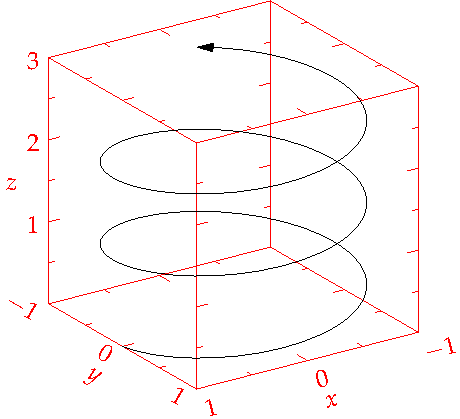
\includegraphics[keepaspectratio]{style-guide/graphics/helix.pdf}}

}

\caption{This is a margin figure. The helix is defined by
\(x = \cos(2\pi z)\), \(y = \sin(2\pi z)\), and \(z = [0, 2.7]\). The
figure was drawn using Asymptote.}

\end{figure}%

Full page-width figures and tables may be placed using the
\texttt{column:\ page} directive.

\begin{figure*}

{\centering \pandocbounded{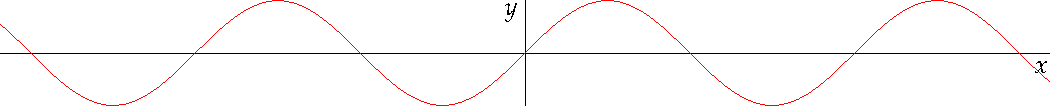
\includegraphics[keepaspectratio]{style-guide/graphics/sine.pdf}}

}

\caption{This graph shows \(y = \sin x\) from about \(x = [-10, 10]\).
\emph{Notice that this figure takes up the full page width.}}

\end{figure*}%

\begin{figure}

{\centering \pandocbounded{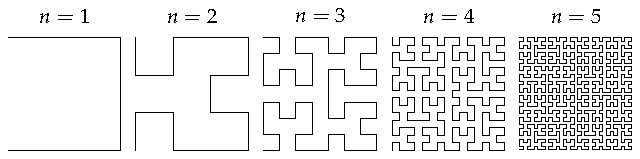
\includegraphics[keepaspectratio]{style-guide/graphics/hilbertcurves.pdf}}

}

\caption{Hilbert curves of various degrees \(n\). \emph{Notice that this
figure only takes up the main textblock width.}}

\end{figure}%

Table (\textbf{tbl:normaltab?}) shows a table created with standard
Quarto table syntax. Notice the lack of vertical rules---they serve only
to clutter the table's data.

\begin{longtable}[]{@{}ll@{}}
\caption{Dimensions of the various margins used in the Tufte-handout
class \{\#tbl:normaltab\}}\tabularnewline
\toprule\noalign{}
Margin & Length \\
\midrule\noalign{}
\endfirsthead
\toprule\noalign{}
Margin & Length \\
\midrule\noalign{}
\endhead
\bottomrule\noalign{}
\endlastfoot
Paper width & 8½ inches \\
Paper height & 11 inches \\
Textblock width & 6½ inches \\
Textblock/sidenote gutter & ⅜ inches \\
Sidenote width & 2 inches \\
\end{longtable}

\section{Typography}\label{sec:typography}

\subsection{Typefaces}\label{sec:typefaces}

If the Palatino, Helvetica, and Bera Mono typefaces are installed, this
style will use them automatically. Otherwise, we'll fall back on the
Computer Modern typefaces.

\subsection{Letterspacing}\label{sec:letterspacing}

This document class includes improvements for letterspacing. When
setting strings of ALL CAPS or small caps, the letterspacing---that is,
the spacing between the letters---should be increased
slightly(Bringhurst 2005).

\section{Document Class Options}\label{sec:options}

The \texttt{tufte-book} class is based on the LaTeX \texttt{book}
document class. Therefore, you can pass any of the typical book options.
There are a few options that are specific to the \texttt{tufte-book}
document class, however.

The \texttt{a4paper} option will set the paper size to A4 instead of the
default US letter size.

The \texttt{sfsidenotes} option will set the sidenotes and title block
in a sans serif typeface instead of the default roman.

The \texttt{twoside} option will modify the running heads so that the
page number is printed on the outside edge (as opposed to always
printing the page number on the right-side edge in \texttt{oneside}
mode).

The \texttt{symmetric} option typesets the sidenotes on the outside edge
of the page. This is how books are traditionally printed, but is
contrary to Tufte's book design which sets the sidenotes on the right
side of the page. This option implicitly sets the \texttt{twoside}
option.

The \texttt{justified} option sets all the text fully justified (flush
left and right). The default is to set the text ragged right. The body
text of Tufte's books are set ragged right. This prevents needless
hyphenation and makes it easier to read the text in the slightly
narrower column.

\chapter{Customizing Tufte-LaTeX}\label{ch:customizing}

The Tufte-LaTeX document classes are designed to closely emulate Tufte's
book design by default. However, each document is different and you may
encounter situations where the default settings are insufficient. This
chapter explores many of the ways you can adjust the Tufte-LaTeX
document classes to better fit your needs.

\section{Numbered Section Headings}\label{sec:numbered-sections}

While Tufte dispenses with numbered headings in his books, if you
require them, they can be enabled by setting the
\texttt{number-sections:\ true} option in the YAML header.

\section{Changing the Paper Size}\label{sec:paper-size}

The Tufte-LaTeX classes currently provide support for different paper
sizes through the \texttt{papersize} option in the YAML header.

\chapter{Compatibility Issues}\label{ch:compatibility}

When switching an existing document from one document class to a
Tufte-LaTeX document class, a few changes to the document may have to be
made.

\section{Converting from article to
tufte-handout}\label{converting-from-article-to-tufte-handout}

Certain heading levels are not supported:
\texttt{\textbackslash{}subsubsection} and
\texttt{\textbackslash{}subparagraph}.

\section{Converting from book to
tufte-book}\label{converting-from-book-to-tufte-book}

Similar restrictions apply for the book class conversion.

\chapter*{References}\label{references-1}
\addcontentsline{toc}{chapter}{References}

\phantomsection\label{refs}
\begin{CSLReferences}{1}{0}
\bibitem[\citeproctext]{ref-Bringhurst2005}
Bringhurst, Robert. 2005. \emph{The Elements of Typography}. 3.1 ed.
Hartley \& Marks.

\bibitem[\citeproctext]{ref-Tufte1990}
Tufte, Edward R. 1990. \emph{Envisioning Information}. Cheshire,
Connecticut: Graphics Press.

\bibitem[\citeproctext]{ref-Tufte1997}
---------. 1997. \emph{Visual Explanations}. Cheshire, Connecticut:
Graphics Press.

\bibitem[\citeproctext]{ref-Tufte2001}
---------. 2001. \emph{The Visual Display of Quantitative Information}.
Cheshire, Connecticut: Graphics Press.

\bibitem[\citeproctext]{ref-Tufte2006}
---------. 2006. \emph{Beautiful Evidence}. First. Graphics Press,
{LLC}.

\end{CSLReferences}


\backmatter


\end{document}
